\documentclass[12pt,
border=1pt]{standalone}
\usepackage{pgfplots}
\usepackage{amsmath}
\usepackage{amssymb}

\pgfplotsset{compat=newest,
	width=6cm, height=5cm,
	xtick pos=left, ytick pos=left,
	%            scaled x ticks=real:1e-6,
}
% Kernel 2 FP64
\begin{document}
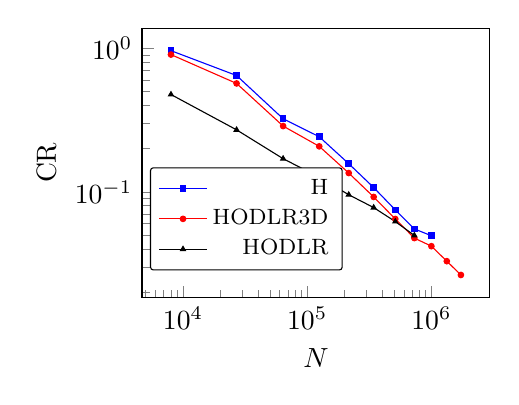
\begin{tikzpicture}[every mark/.append style={mark size=1pt}]
	\begin{axis}[xlabel={$N$},
	ylabel={CR},
%		legend pos=south east,
		legend style={
                at={(0.3,0.1)},
               anchor=south,
               legend columns=1,
               cells={anchor=east},
               font=\footnotesize,
               rounded corners=1pt,
               },
		xmode = log,
	    ymode = log,
	   % xmin = 1e3,
	   % xmax = 1e6,
	   % ymin = 1e-10,
	   % ymax = 1e-0,
	   % xtick={1e-10, 1e-8, 1e-6,  1e-4,  1e-2},
	   % ytick={1e-8, 1e-6,  1e-4,  1e-2, 1e-0}
		]

		%Vaishnavi
		\addplot[
		color=blue,
		mark=square*,
		] coordinates {
(8000,9.616210e-01)
(27000,6.454190e-01)
(64000,3.228080e-01)
(125000,2.419280e-01)
(216000,1.570840e-01)
(343000,1.071640e-01)
(512000,7.489180e-02)
(729000,5.520650e-02)
(1000000,4.948590e-02)
		};
		%Zhao
		\addplot[
		color=red,
		mark=*,
		] coordinates {
(8000,9.030500e-01)
(27000,5.686530e-01)
(64000,2.871140e-01)
(125000,2.073970e-01)
(216000,1.352020e-01)
(343000,9.217040e-02)
(512000,6.475690e-02)
(729000,4.765240e-02)
(1000000,4.184530e-02)
(1331000,3.291040e-02)
(1728000,2.638050e-02)
		};
\addplot[
		color=black,
		mark=triangle*,
		] coordinates {
(8000,4.761110e-01)
(27000,2.702150e-01)
(64000,1.701760e-01)
(125000,1.263950e-01)
(216000,9.544790e-02)
(343000,7.772110e-02)
(512000,6.211540e-02)
(729000,4.972400e-02)
		};
		\legend{H, HODLR3D, HODLR}	\end{axis}
\end{tikzpicture}
\end{document}